% Created 2018-04-10 mar 12:18
\documentclass[a4paper]{scrartcl}
\usepackage[utf8]{inputenc}
\usepackage[T1]{fontenc}
\usepackage{fixltx2e}
\usepackage{graphicx}
\usepackage{longtable}
\usepackage{float}
\usepackage{wrapfig}
\usepackage{rotating}
\usepackage[normalem]{ulem}
\usepackage{amsmath}
\usepackage{textcomp}
\usepackage{marvosym}
\usepackage{wasysym}
\usepackage{amssymb}
\usepackage{hyperref}
\tolerance=1000
\usepackage{khpreamble}
\author{Kjartan Halvorsen}
\date{Due Friday 2018-04-20}
\title{Computerized control - homework 6}
\hypersetup{
  pdfkeywords={},
  pdfsubject={},
  pdfcreator={Emacs 24.5.1 (Org mode 8.2.10)}}
\begin{document}

\maketitle

\section*{Preliminary report on the project and plan for the work}
\label{sec-1}

Please prepare a written preliminary report about your work on the project. The report should contain
\begin{enumerate}
\item \textbf{Design of the necessary analog circuits:}
\begin{enumerate}
\item Antialiasing filter (low pass Bessel filter). In order to find a reasonable value of the sampling period \(h\), you can make use of the step response in the figure below (by previous students Pedro de la Torre, Jorge Ramirez, Jorge Barrutia, Miguel Rubio). 
\begin{center}
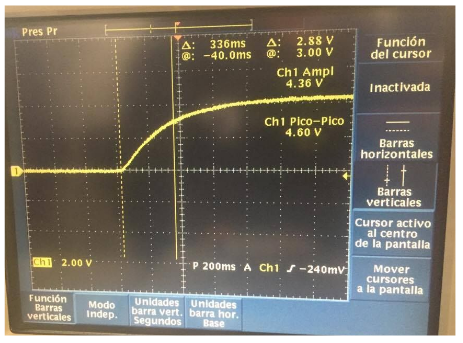
\includegraphics[width=0.8\linewidth]{../figures/step-response-oscilloscope.png}
\end{center}
\item Signal conditioner (motor driver) to convert a 0-5V signal from Arduino output channel to signal -5V - +5V for driving the dc motor in both directions.
\item Signal conditioner to convert zero-mean signal from anti-aliasing filter to signal in range 0-5V for input to Arduino.
\end{enumerate}
\item \textbf{A detailed plan of the work} needed to complete the project and finish the report. Break the work up in a number of suitable tasks and \textbf{provide for each task}
\begin{enumerate}
\item A description
\item Time required to complete the task
\item Deadline to accomplish the task and scheduled times to work on the task.
\item Responsible group member
\end{enumerate}
You could for instance visualize the plan in a \href{https://es.wikipedia.org/wiki/Diagrama_de_Gantt}{Gantt chart}
\end{enumerate}
% Emacs 24.5.1 (Org mode 8.2.10)
\end{document}